\documentclass[a4paper,11pt,twoside]{article}
%\documentclass[a4paper,11pt,twoside,se]{article}

\usepackage{UmUStudentReport}
\usepackage{verbatim}   % Multi-line comments using \begin{comment}
\usepackage{courier}    % Nicer fonts are used. (not necessary)
\usepackage{pslatex}    % Also nicer fonts. (not necessary)
\usepackage[pdftex]{graphicx}   % allows including pdf figures
\usepackage{listings}
\usepackage{pgf-umlcd}
%\usepackage{lmodern}   % Optional fonts. (not necessary)
%\usepackage{tabularx}
%\usepackage{microtype} % Provides some typographic improvements over default settings
%\usepackage{placeins}  % For aligning images with \FloatBarrier
%\usepackage{booktabs}  % For nice-looking tables
%\usepackage{titlesec}  % More granular control of sections.

% DOCUMENT INFO
% =============
\department{Department of Computing Science}
\coursename{Object-Oriented Programming Methodology 7.5 p}
\coursecode{5DV133}
\title{OU3 Sensor Network}
\author{Johan Eklund ({\tt{kv03jed@cs.umu.se}}) \\ 
Tommie Lindberg ({\tt{c15tlg@cs.umu.se}}) \\
Jakob Lundin ({\tt{c14jln@cs.umu.se}}) \\
Lorenz Gerber ({\tt{dv15lgr@cs.umu.se}}, {\tt{lozger03@student.umu.se}})
}
\date{2016-05-04}
%\revisiondate{2016-01-18}
\instructor{Anders Broberg \\ Niklas Fries \\ Adam Dahlgren \\
  Jonathan Westin \\ Erik Moström \\ Alexander Sutherland}


% DOCUMENT SETTINGS
% =================
\bibliographystyle{plain}
%\bibliographystyle{ieee}
\pagestyle{fancy}
\raggedbottom
\setcounter{secnumdepth}{2}
\setcounter{tocdepth}{2}
%\graphicspath{{images/}}   %Path for images

\usepackage{float}
\floatstyle{ruled}
\newfloat{listing}{thp}{lop}
\floatname{listing}{Listing}



% DEFINES
% =======
%\newcommand{\mycommand}{<latex code>}

% DOCUMENT
% ========
\begin{document}
\lstset{language=C}
\maketitle
\thispagestyle{empty}
\newpage
\tableofcontents
\thispagestyle{empty}
\newpage

\clearpage
\pagenumbering{arabic}

\section{Introduction} 
The assignment was described on the course homepage
\cite{sensornetwork}. 

\subsection{General Design Considerations}
In object oriented software design, it is common to build 
a model representation of the real world system \cite{roleplay} by
defining classes the correspond to the real world systems' entities.  
Here the real world system is a sensor network as described in
Braginsky and Estrin \cite{braginsky2002}. The realworld entities
modelled in this assignment can be classified in two main groups: Physical
components such as the sensor nodes and non-physical ones, information packages
travelling the network, such as the queries and agents. Further, a third type, 
the environment entity simulates the real surrounding.



\textit{Unified Modelling Language}
(\textit{UML}) and \textit{Class Responsibility Collaborator}
(\textit{CRC}) diagrams were composed according to Börstler
\cite{roleplay}. The theory of rumour routing is described by Braginsky
\cite{braginsky2002}. Horstman was used as Java language reference
\cite{horstman2014}.


\section{Classes Responsibilities and Collaborations}
The Class Responsibilities and Collaborations (CRC) diagaram is shown
in figure \ref{fig:crc}.
 
\begin{figure}
\centering
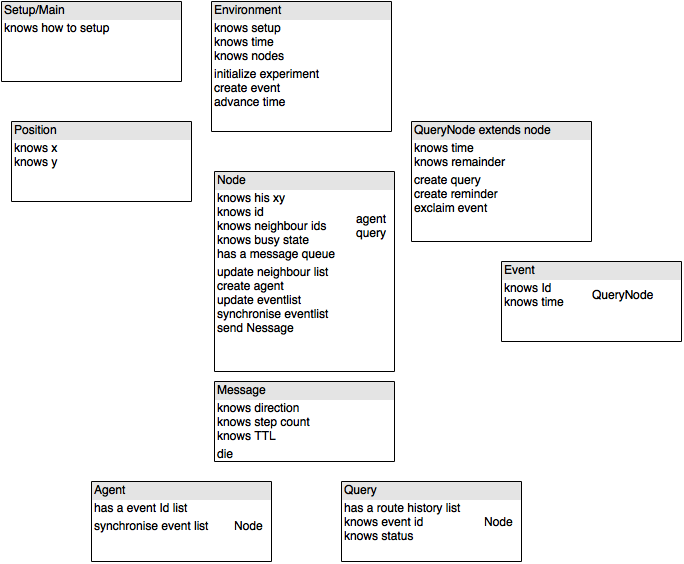
\includegraphics[width=\textwidth]{crc.png}
\caption{This is the crc diagram}
\label{fig:crc}
\end{figure}

\section{Unified Modelling Language Class Diagram}

\begin{figure}
\centering
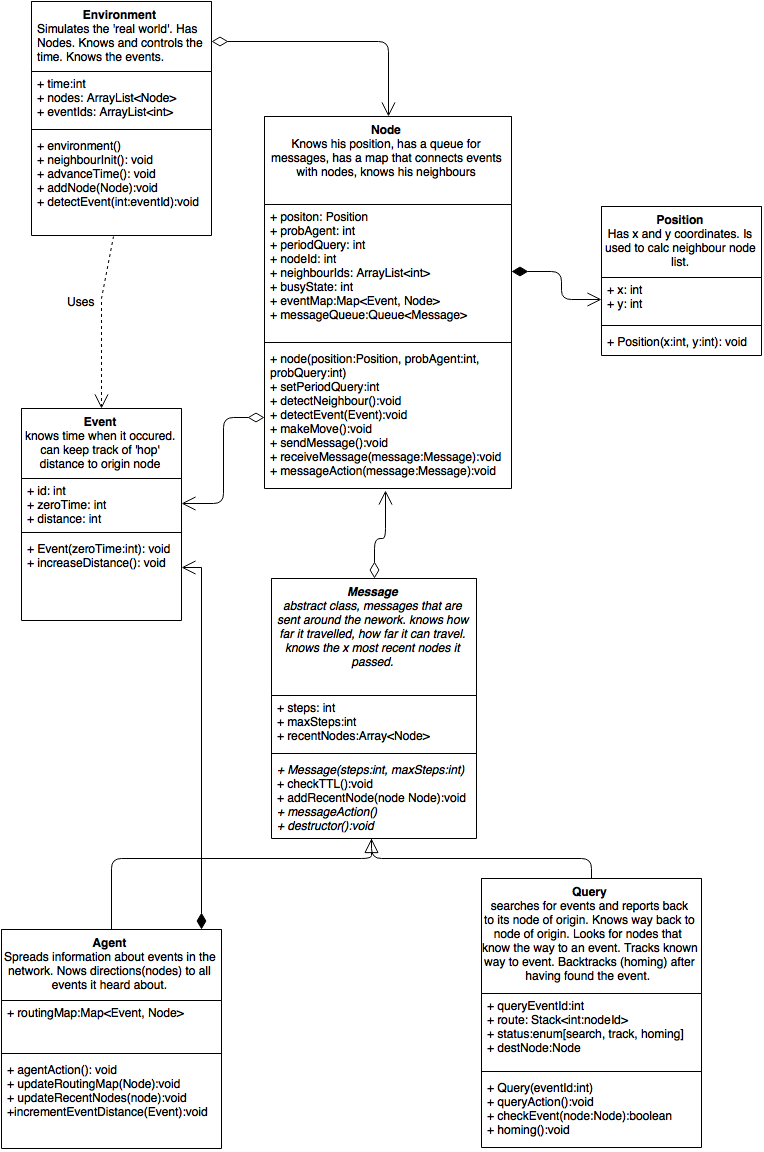
\includegraphics[width=\textwidth]{uml.png}
\caption{This is the uml diagram}
\label{fig:uml}
\end{figure}


\section{Initialization and State Stepping}
\subsection{Overview}
First parameters that are needed to create nodes have to be determined.
That includes the position, and the probability to create agents after
an event happens. Then nodes can be created and
positioned. Afterwards, nodes have to be initialized to know their
neighbours. According to Braginsky and Estrin \cite{braginsky2002},
composing the neighbour list could happend either as an initial
startup phase, but if nodes are assumed non-static, also
continuous. Here nodes were assumed static. Finally, experimental
parameters for the environment need to be initialized. These are
parameters such as which nodes will create queries and in which
frequency. But also the probabilty of events and how the node to
experience them is selected. 

Setup/Main instantiates the Environment, then instantiates the Nodes
with coordinates and places them in the environment. On
instantiation, the probability for agent creation is set as attribut
in each node.

In each time step, the environment cycles through all
nodes. At each node a nubmer of possbile actions are considered and if
viable performed. These include: creating an agent, creating a query,
receiving a query, receiving an agent, sending a query, sending an
agent.

From the description, it is not clear if creating an agent or a query
involves also sending it in the same time step. This behaviour needs
to be defined. What happens if a node has one or more messages in the
queue, detects an event and is supposed to send an agent. Does the
agent end up in the queue? Same question for a query.

First random generation of an event, then to handle the messages
(agents and queries). Messages are put in a queue in the node. If
a node has either sent, received, or instantiated a new message, a
busy flag is set, so that no other operation from outside
can be accepted.   

\begin{verbatim}
Main
{

  //Globals
  NODES_X = 50
  NODES_Y = 50
  NO_NODES = NODOES_X * NODES_Y
  NEW_EVENTS = 0.0001
  NODE_RANGE = 
  TTL_AGENT = 50
  TTL_QUERY = 50
  QUERY_NODES = 4
  QUERY_PERIODICITY = 400

  // Create Environment
  myEnv = Environment()


  // Create and position Nodes
  For (x = 1:NODES_X)
  {
    For (y = 1 -> NODES_Y)
    {
      myEnv.addNode(Node(Position(x, y),0.5, NULL))
    }
  }

  // Set Query nodes
  queryNodeIds[] = sample(1, NO_NODES, QUERY_NODES)
  For (i = 1:QUERY_NODES)
  {
    myEnv.nodes.getNode(queryNodeIds[i]).setPeriodQuery(QUERY_PERIODICITY)
  }


  // Create Neighbour list
  // For every node
  For(nodes_create_list = 1:NO_NODES)
  {
    // create neighbour list 

    For(nodes_check_distance = 1:NO_NODES)
    {
      // detectNeighbour checks distance and adds node id to neighbour
if in range

      myEnv.nodes.getNode(nodes_create_list).detectNeighbour(myEnv.nodes.getNode(nodes_check_distance))
    }
  }


  //
  For(timesteps 1:10000)
  {
    myEnv.advanceTime()
  }
}
\end{verbatim}

bla bla bla

\begin{verbatim}

Class Environment
{

  int time
  ArrayList<Node> nodes

  Environment(){
    
    new Environment
  }

  advanceTimer(){
    //id 1:NO_NODES){
    detectEvent(node_id)
    makeMove(node_id)
  }
}
\end{verbatim}

bla bla bal

\begin{verbatim}

Class Node
{
  detectEvent()
  {

  randomFunction(PROB_NEW_EVENTS){
  eventMap.add(Event(), self.nodeId)
  }

  makeMove()
  {

  // new event? (detectEvent())
    // Random function to create Agent
  // New Query?
    //put query on message queue
  // Do we have a message on Message Queue
    // Do messageAction()
    // BusyState, have we already done our move
    // if we can send, send message

  // reduce queryPeriodicityCounter by 1
  }

  sendMessage()
  {
  // find out receiver
    // Check type of message
      // if message "Query"
        //check Query status (search/track/homing)
    // is receiver free 
      // send message
      // call receiveMessage of receiver
      // set BusyState
  }


  receiveMessage()
  {
  // Add message to messageQueue
  // set BusyState
  // is Message Agent?
    // call Event Increment distance 
  }
}

\end{verbatim}

bla bla bla

\begin{verbatim}

Class Message
{

  messageAction()

}


Class Query
{

  queryAction()
  {
  // checkMode

    //// Search Mode
    // check eventId in Node eventMap
    // if path found
      // switch mode

    //// Track Mode
    // check destination reached
      // switch mode

    //// Homing Mode
    // check start reached / is stack empty
      // exclaim Event(Node Position, zeroTime, NodeId)
  }
}


Class Agent
{
  agentAction()
  {

  // compare and adjust eventMaps between agent and node
  // check TTL
   // decrement TTL
  }

}

\end{verbatim}






\section{Testing Framework}


\addcontentsline{toc}{section}{\refname}
\bibliography{references}

\end{document}
 
